% ****** Start of file aipsamp.tex ******
%
%   This file is part of the AIP files in the AIP distribution for REVTeX 4.
%   Version 4.1 of REVTeX, October 2009
%
%   Copyright (c) 2009 American Institute of Physics.
%
%   See the AIP README file for restrictions and more information.
%
% TeX'ing this file requires that you have AMS-LaTeX 2.0 installed
% as well as the rest of the prerequisites for REVTeX 4.1
%
% It also requires running BibTeX. The commands are as follows:
%
%  1)  latex  aipsamp
%  2)  bibtex aipsamp
%  3)  latex  aipsamp
%  4)  latex  aipsamp
%
% Use this file as a source of example code for your aip document.
% Use the file aiptemplate.tex as a template for your document.
\documentclass[%
notitlepage,
 %reprint,%
%author-year,%
%author-numerical,%
%draft,
]{revtex4-1}

\usepackage{graphicx}% Include figure files
\usepackage{dcolumn}% Align table columns on decimal point
\usepackage{bm}% bold math

% packages added by Anand
\usepackage{subfig}
\usepackage{color}
\usepackage{amsmath}
\usepackage{amssymb}
\usepackage{xspace}
\usepackage{multirow}
\usepackage{bm}
%\usepackage[mathlines]{lineno}% Enable numbering of text and display math
%\linenumbers\relax % Commence numbering lines
\include{custom_commands}
\everymath{\displaystyle}


% comment the following lines to see figures
%\usepackage{ifdraft}
%\ifdraft{\renewcommand{\includegraphics}{\relax}}{\relax}
%\renewcommand{\includegraphics}[2][]{}
%\renewcommand{\subfloat}[0]{}
\usepackage{url}

\begin{document}

\preprint{}

\title[]{One Dimensional Problems}% Force line breaks with \\
%\thanks{Footnote to title of article.}

%\author{Anand Pratap Singh}
%\email{anandps@umich.edu}
%\affiliation{Department of Aerospace Engineering, University of Michigan, Ann Arbor, MI 48109, USA}%

\date{\today}% It is always \today, today,
             %  but any date may be explicitly specified

\begin{abstract}

\end{abstract}

%\pacs{Valid PACS appear here}% PACS, the Physics and Astronomy
                             % Classification Scheme.
%\keywords{Suggested keywords}%Use showkeys class option if keyword
                              %display desired
\maketitle
\subsection{Linear}
\begin{figure}[!h]
	\subfloat[]{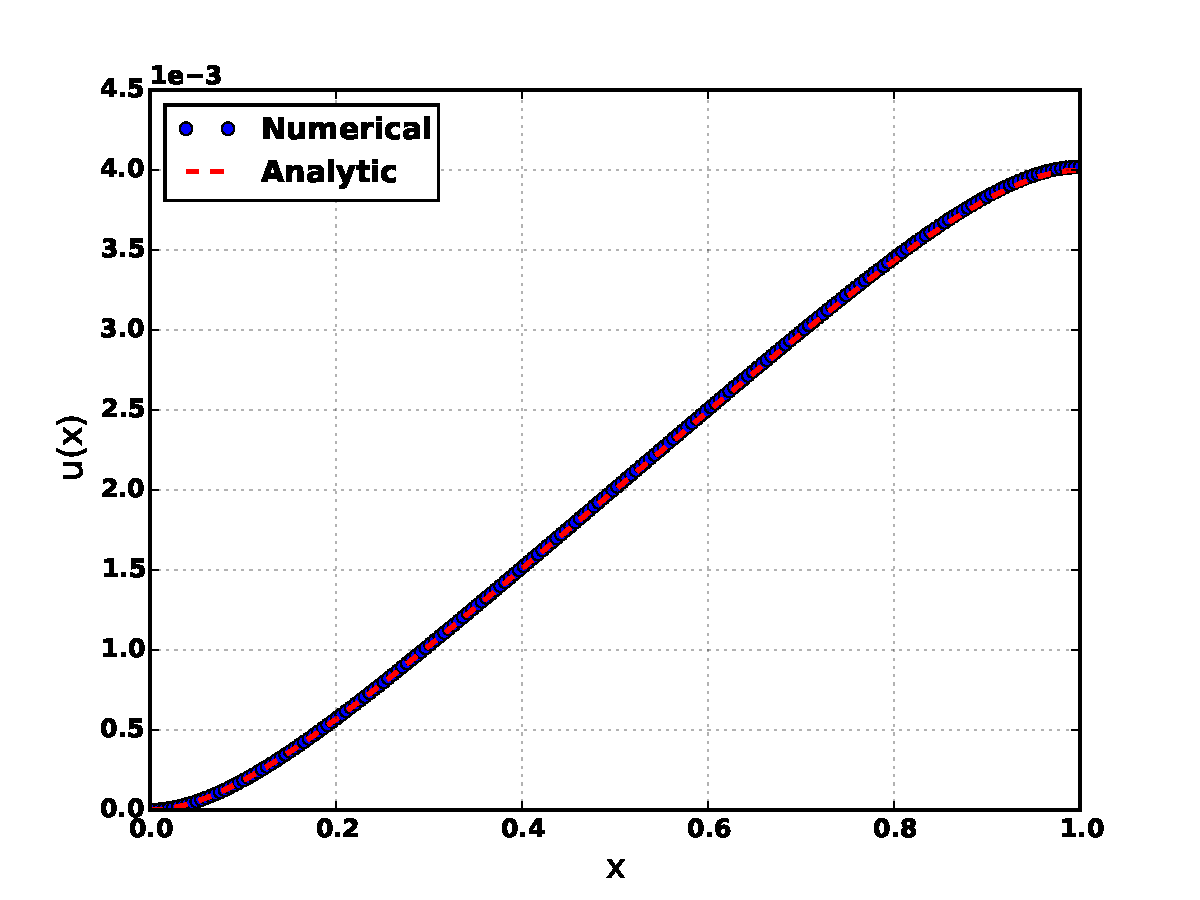
\includegraphics[width=0.45\textwidth]{figures/linear_01/solution.pdf}}
    \subfloat[]{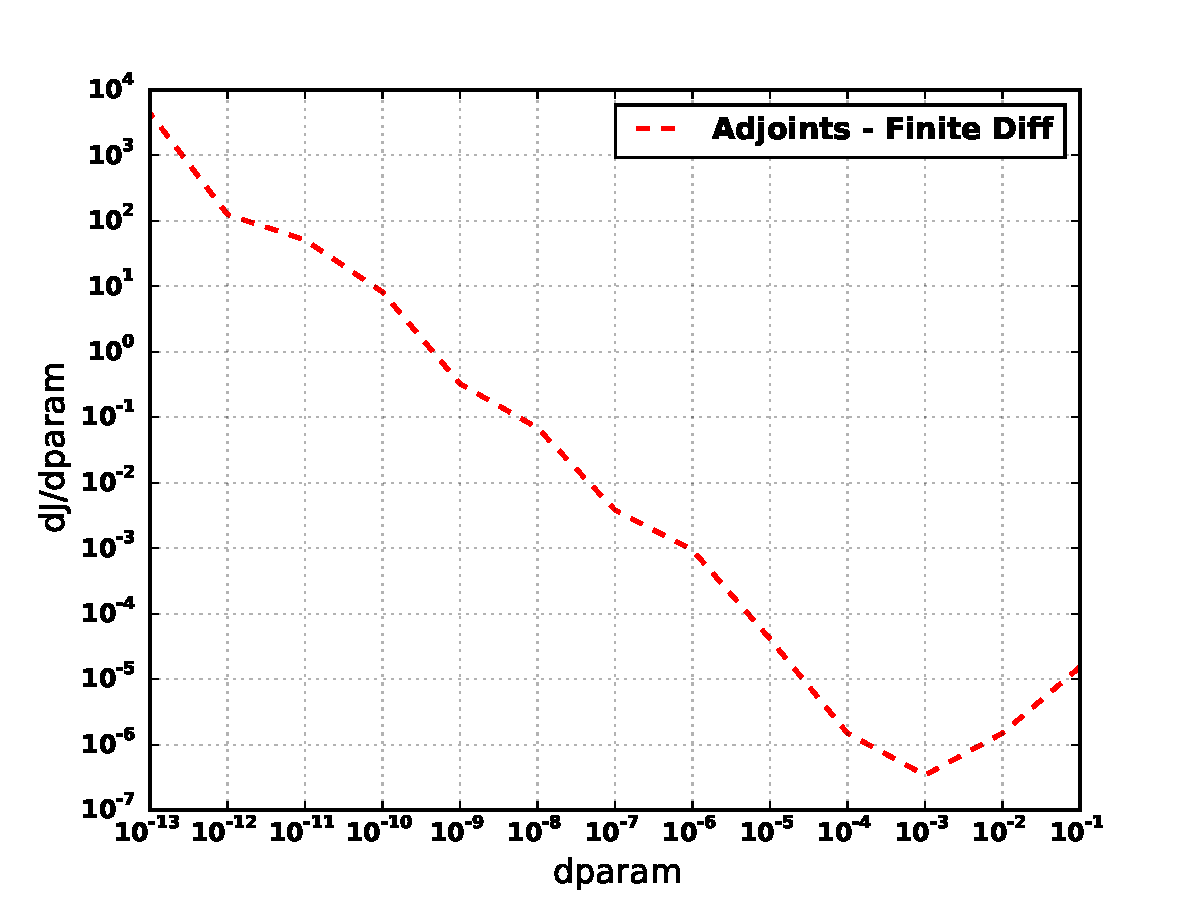
\includegraphics[width=0.45\textwidth]{figures/linear_01/sensitivity.pdf}}
\end{figure}
\subsection{Nonlinear}
\begin{figure}[!h]
	\subfloat[]{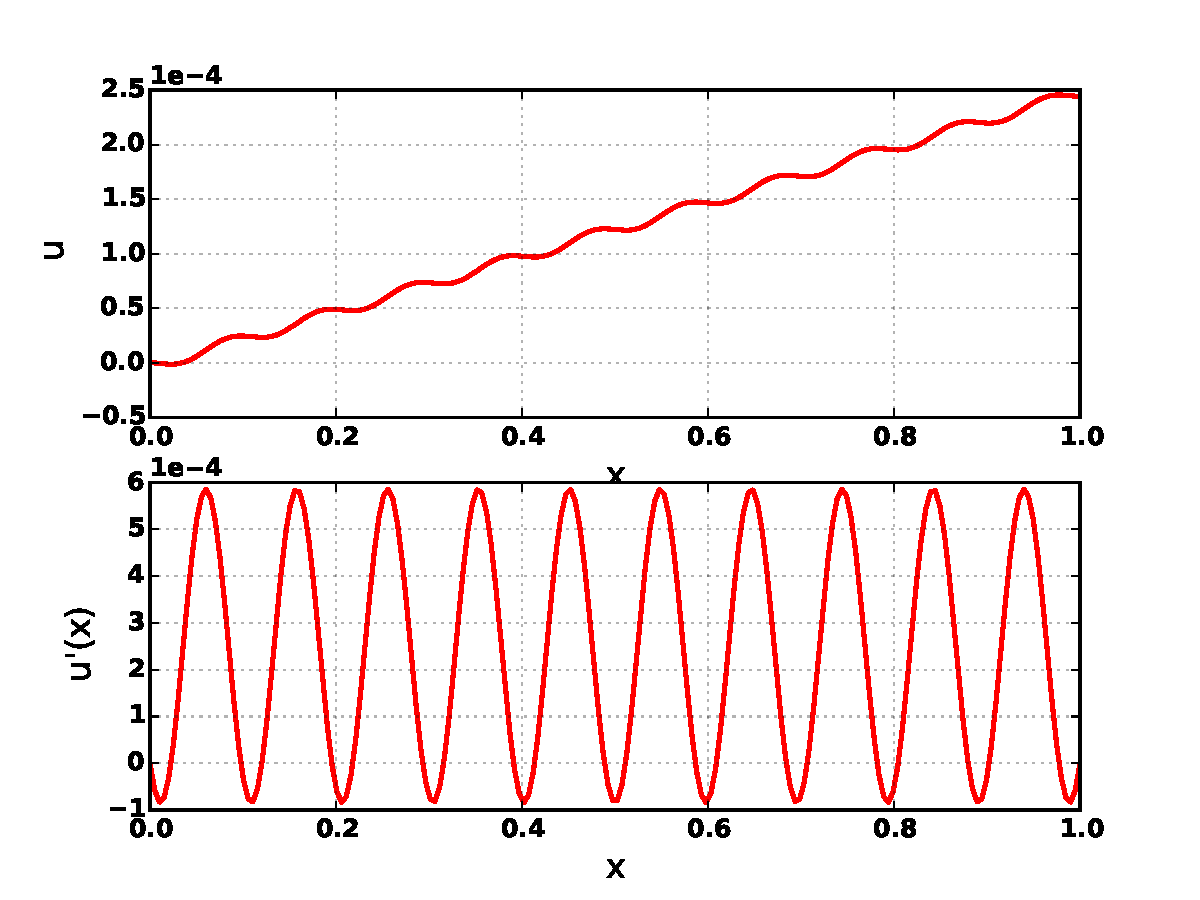
\includegraphics[width=0.45\textwidth]{figures/nonlinear_02/solution.pdf}}
    \subfloat[]{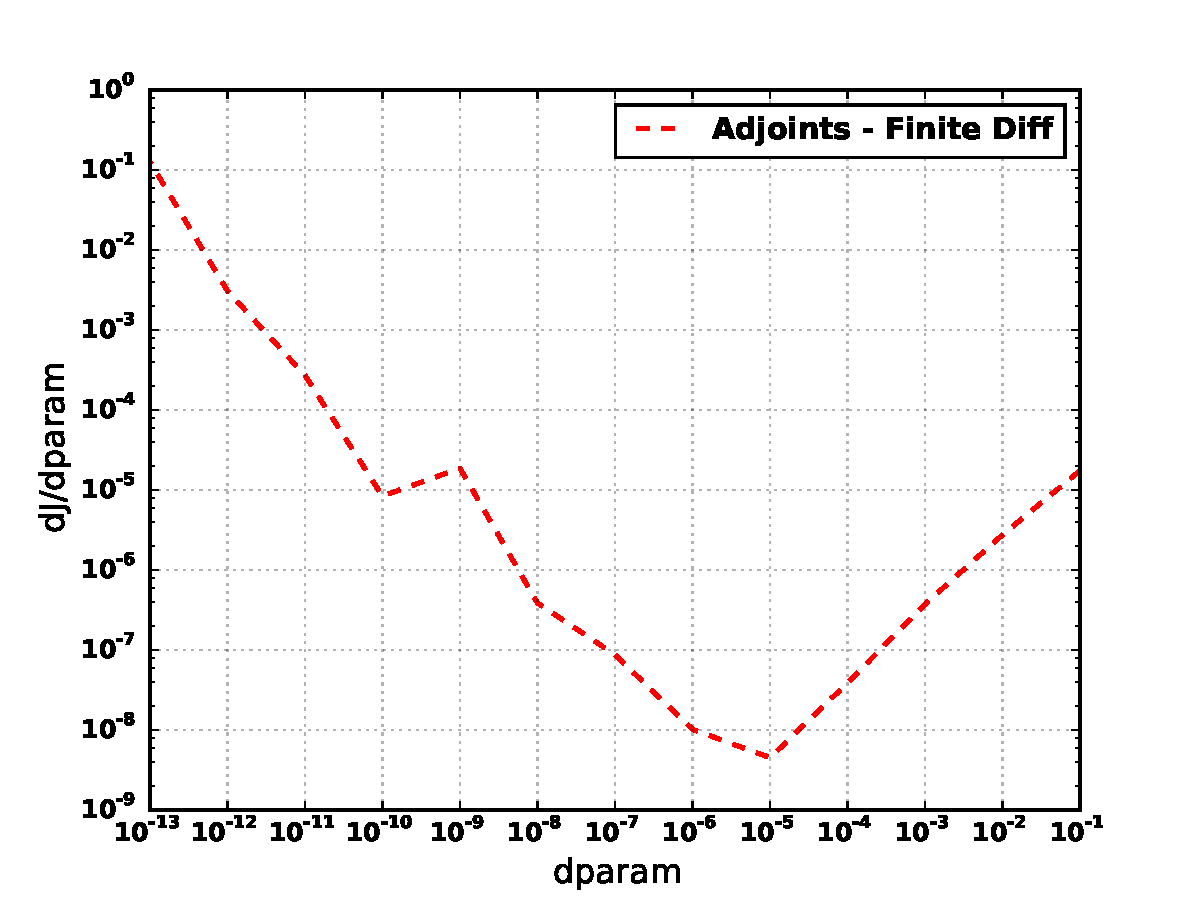
\includegraphics[width=0.45\textwidth]{figures/nonlinear_02/sensitivity.pdf}}
\end{figure}
\subsection{Linear Inversion}
\begin{figure}[!h]
	\subfloat[]{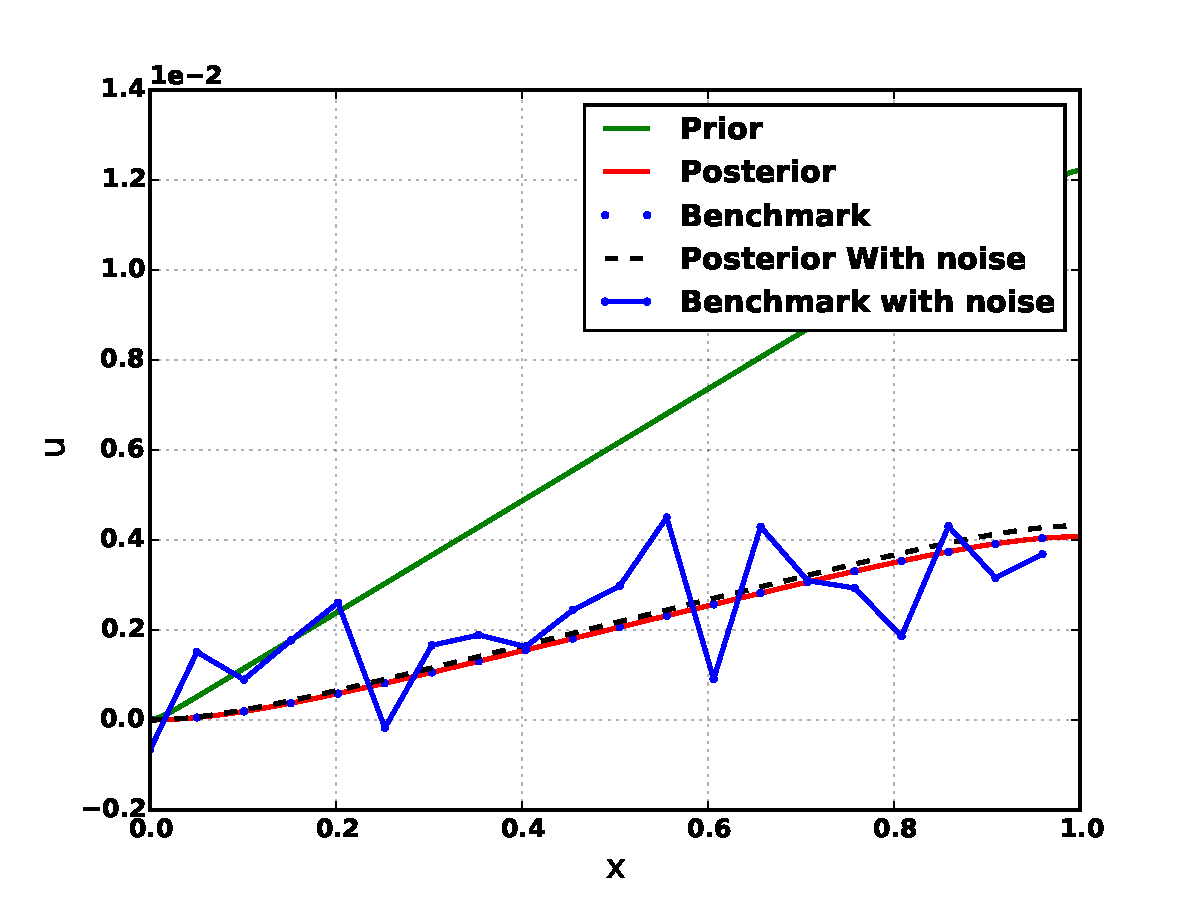
\includegraphics[width=0.45\textwidth]{figures/linear_inverse_03/inverse.pdf}}
    \subfloat[]{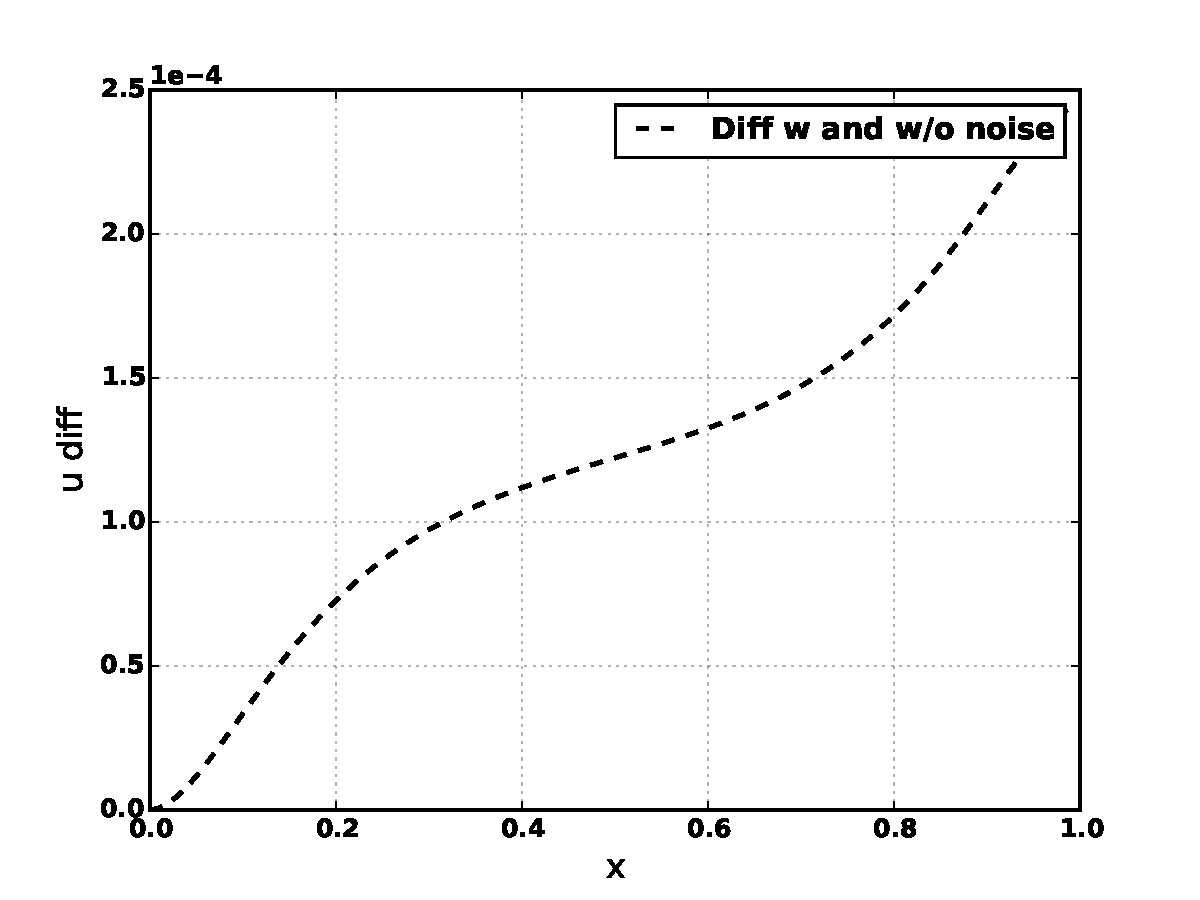
\includegraphics[width=0.45\textwidth]{figures/linear_inverse_03/diff.pdf}}
\end{figure}
\subsection{Nonlinear Inversion}
\appendix
\subsection{Solver}
\end{document}

%
% ****** End of file aipsamp.tex ******
